\documentclass[11pt]{amsart}
%\pagestyle{empty} 
\setlength{\topmargin}{-0.75in} % usually -0.25in
\addtolength{\textheight}{1.25in} % usually 1.25in
\addtolength{\oddsidemargin}{-1.2in}
\addtolength{\evensidemargin}{-1.2in}
\addtolength{\textwidth}{1.9in} %\setlength{\parindent}{0pt}

\newcommand{\normalspacing}{\renewcommand{\baselinestretch}{1.1}\tiny\normalsize}
\normalspacing

% macros
\usepackage{amssymb,xspace,alltt,verbatim}
\usepackage[final]{graphicx}
\usepackage[pdftex,colorlinks=true]{hyperref}
\usepackage{fancyvrb}
\usepackage{tikz}

\newtheorem*{lem*}{Lemma}

\newcommand{\bb}{\mathbf{b}}
\newcommand{\bc}{\mathbf{c}}
\newcommand{\bs}{\mathbf{s}}
\newcommand{\bu}{\mathbf{u}}
\newcommand{\bv}{\mathbf{v}}
\newcommand{\bw}{\mathbf{w}}
\newcommand{\bx}{\mathbf{x}}
\newcommand{\by}{\mathbf{y}}

\newcommand{\bbf}{\mathbf{f}}

\newcommand{\CC}{{\mathbb{C}}}
\newcommand{\RR}{{\mathbb{R}}}
\newcommand{\eps}{\epsilon}
\newcommand{\ZZ}{{\mathbb{Z}}}
\newcommand{\ZZn}{{\mathbb{Z}}_n}
\newcommand{\NN}{{\mathbb{N}}}
\newcommand{\ip}[2]{\mathrm{\left<#1,#2\right>}}

\renewcommand{\Re}{\operatorname{Re}}
\renewcommand{\Im}{\operatorname{Im}}

\newcommand{\Log}{\operatorname{Log}}

\newcommand{\grad}{\nabla}

\newcommand{\ds}{\displaystyle}

\newcommand{\Matlab}{\textsc{Matlab}\xspace}
\newcommand{\Octave}{\textsc{Octave}\xspace}
\newcommand{\pylab}{\textsc{pylab}\xspace}

\newcommand{\prob}[1]{\bigskip\noindent\textbf{#1.} }
\newcommand{\pts}[1]{(\emph{#1 pts})}

\newcommand{\probpts}[2]{\prob{#1} \pts{#2} \quad}
\newcommand{\ppartpts}[2]{\textbf{(#1)} \pts{#2} \quad}
\newcommand{\epartpts}[2]{\medskip\noindent \textbf{(#1)} \pts{#2} \quad}


\begin{document}
\hfill \Large Name:\underline{\phantom{Ed Bueler really really long long long name}}
\medskip

\scriptsize \noindent Math 252 Calculus 2 (Bueler) \hfill Thursday, 7 April 2022
\medskip

\LARGE\centerline{\textbf{Midterm Exam 2}}

\smallskip
\begin{quote}
\large
\textbf{No book, notes, electronics, calculator, or internet access.  100 points possible. 70 minutes maximum.}
\end{quote}

\normalsize
\medskip

\thispagestyle{empty}

\prob{1}  Compute and simplify the improper integrals, or show they diverge.  Use correct limit notation.

\epartpts{a}{5} $\ds \int_0^\infty \frac{x^2\, dx}{1+x^3} = $
\vfill

\epartpts{b}{5} $\ds \int_0^1 \frac{dx}{\sqrt[4]{x}} =$
\vfill

\probpts{2}{5}  Does the following series converge or diverge?  Show your work, including naming any test you use.  (\emph{Hint.}  Previous problem?  Or another test?)
  $$\sum_{n=0}^\infty \frac{n^2}{1+n^3} = \hspace{4.5in}$$
\vfill


\clearpage\newpage
\prob{3}  Do the following series converge or diverge?  Show your work, including naming any test you use.

\epartpts{a}{5}  $\ds \sum_{n=0}^\infty \frac{n+2}{4^n}$
\vfill

\epartpts{b}{5}  $\ds \sum_{n=0}^\infty \frac{(-1)^n 3^n}{4^n}$
\vfill

\epartpts{c}{5}  $\ds \sum_{n=2}^\infty \frac{(-1)^n}{\ln n}$
\vfill


\clearpage\newpage
\epartpts{d}{5}  $\ds \sum_{n=1}^\infty \frac{n!}{n^n}$
\vfill

\epartpts{e}{5}  $\ds \sum_{n=1}^\infty \frac{(\cos n)^2}{n^2}$
\vfill

\probpts{4}{5}  For one of the five series in problem \textbf{3}, it is possible to compute the value of the infinite series.  Which one?  Explain why, and compute the value.
\vfill


\clearpage\newpage
\prob{5}  Consider the infinite series $\ds 1-\frac{1}{2}+\frac{1}{3}-\frac{1}{4}+\frac{1}{5} - \dots$

\epartpts{a}{5}  Write the series using sigma ($\Sigma$) notation.
\vspace{2.0in}

\epartpts{b}{5}  Compute and simplify $S_4$, the partial sum of the first four terms.
\vspace{2.0in}

\newcommand{\threeopts}{{\small \hspace{-6mm} $\begin{matrix} \text{\textsc{converges}} \\ \text{\textsc{absolutely}} \end{matrix}$ \qquad\qquad $\begin{matrix} \text{\textsc{converges}} \\ \text{\textsc{conditionally}} \end{matrix}$ \qquad\qquad \textsc{diverges}} \bigskip}

\probpts{6}{5}  Does the series $\ds \sum_{n=1}^\infty \frac{(-1)^n}{n^3}$ converge absolutely, conditionally, or neither (diverge)?  Show your work and circle one answer. 
\vfill

\threeopts


\clearpage\newpage
\prob{7}  By any method, write a power series for the following functions.  Show your work.

\epartpts{a}{5}  $\ds \frac{1}{1+2x}$
\vspace{3.0in}

\epartpts{b}{7}  $\ds \arctan x$

\medskip
\noindent (\emph{Hint.} Integrate a series derived from the geometric series.)
\vfill


\clearpage\newpage
\prob{8}  Find the interval of convergence of the following power series.

\epartpts{a}{7}  $\ds \sum_{n=1}^\infty \frac{x^n}{n 2^n}$
\vfill

\epartpts{b}{5}  $\ds \sum_{n=1}^\infty (n-1)!\,x^n$
\vfill


\clearpage\newpage
\probpts{9}{9} Find the Taylor series of $\ds f(x)=\frac{1}{x}$ at basepoint $a=2$.
\vfill

\probpts{10}{7} Use the midpoint rule with $n=2$ subintervals to estimate $\ds \int_0^1 x^3\,dx$.  Simplify your result.
\vspace{2.5in}


\clearpage\newpage
\probpts{Extra Credit}{3}  Recall the famous Maclaurin series $\ds e^x = \sum_{n=0}^\infty \frac{x^n}{n!}$.  Suppose I put $x=-\frac{1}{2}$ in this power series.  In fact, suppose I compute the 10th partial sum $\ds S_{10}=\sum_{n=0}^{10} \frac{(-1/2)^n}{n!}$.  I observe, using Matlab, that it gives more than 10 digits of accuracy in approximating $e^{-1/2}=\frac{1}{\sqrt{e}}$.  Explain why, using a known fact about remainders.
\vfill

\noindent \hrule
\begin{center}
\small
\bigskip
\textsc{blank space}
\end{center}
\vspace{3.0in}


\clearpage\newpage
\large\centerline{\textbf{Summary of Convergence Tests}}
\normalsize

\begin{center}
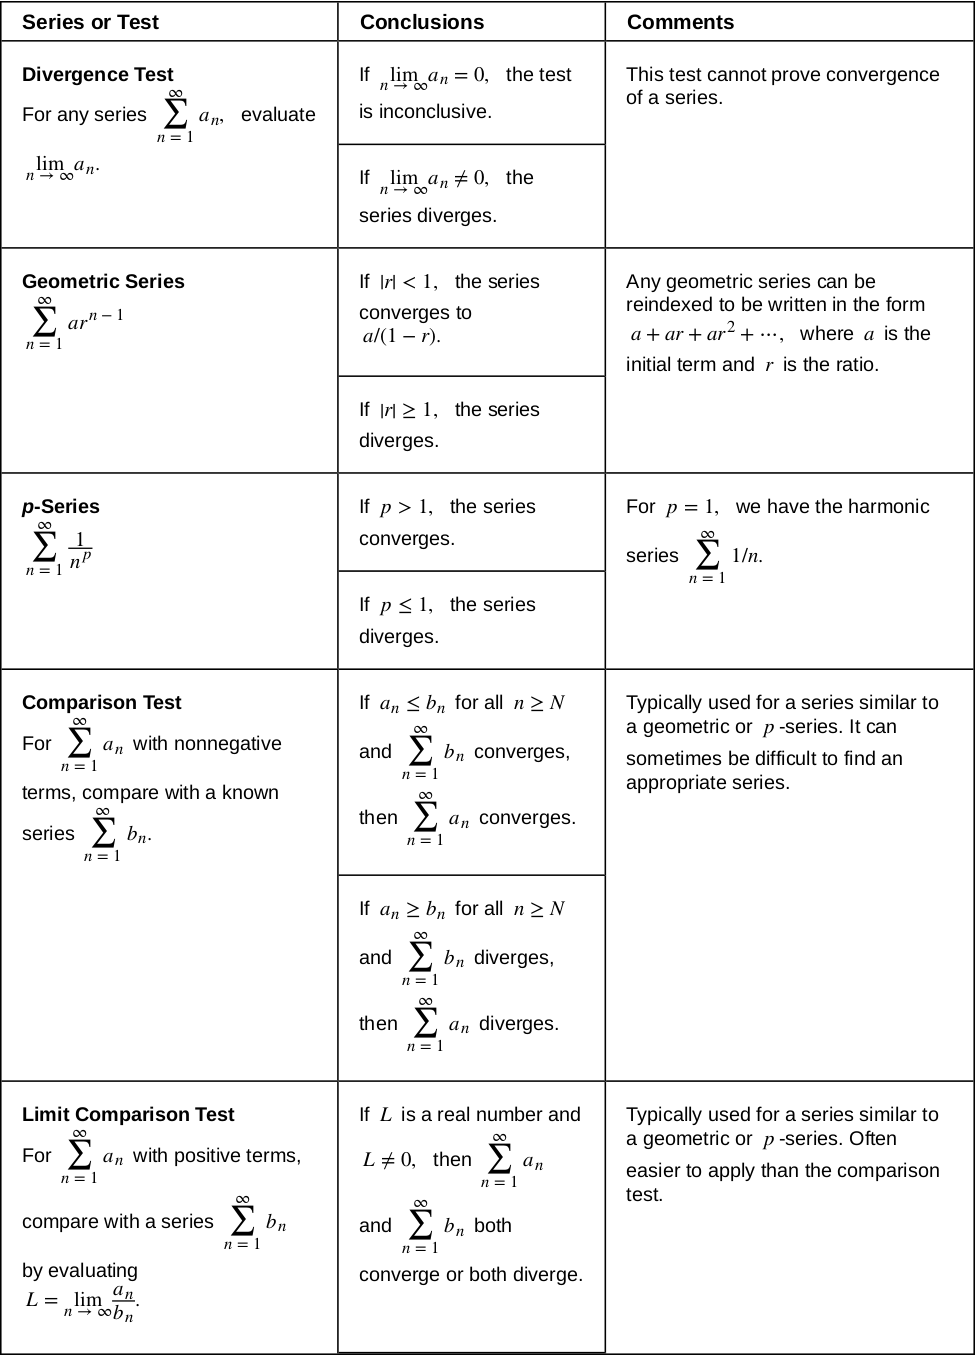
\includegraphics[width=0.95\textwidth]{figs/serieshandoutA.png}
\end{center}
\vfill


\clearpage\newpage
\begin{center}
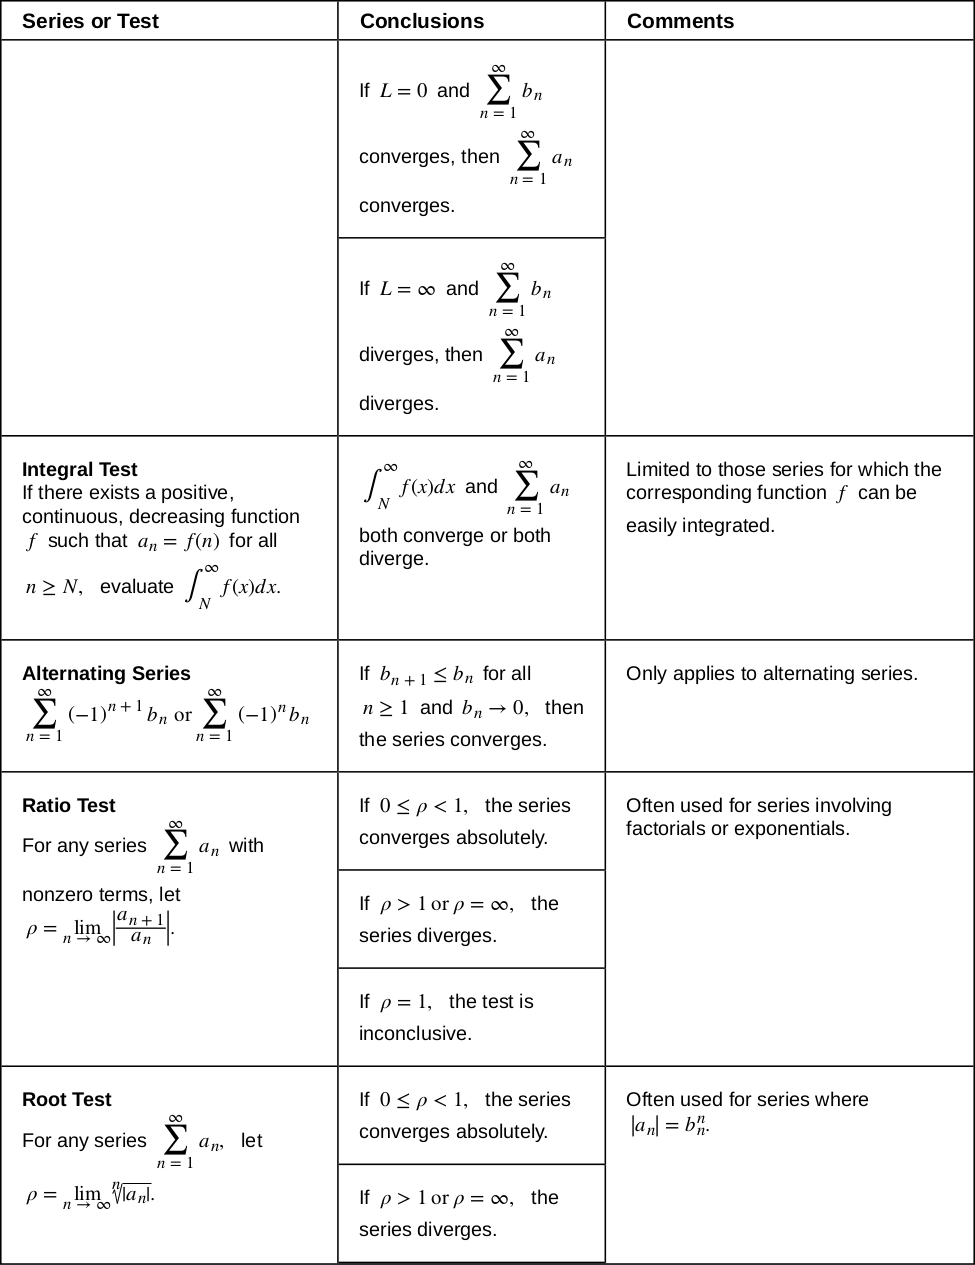
\includegraphics[width=0.95\textwidth]{figs/serieshandoutB.png}

\vspace{-2mm}

\includegraphics[width=0.95\textwidth]{figs/serieshandoutC.png}
\end{center}
\vfill

\end{document}
